\begin{savequote}[10cm] % this sets the width of the quote
\sffamily
The message itself was unknown to Salo. It had been prepared by what Salo described to Rumfoord as, ``A kind of university--only nobody goes to it. There aren't any buildings, isn't any faculty. Everybody's in it and nobody's in it. It's like a cloud that everybody has given a little puff of mist to, and then the cloud does all the heavy thinking for everybody. I don't mean there's really a cloud. I just mean it's something like that. If you don't understand what I'm talking about, Skip, there's no sense in trying to explain it to you. All I can say is, there aren't any meetings"

\qauthor{Kurt Vonnegut -- The Sirens of Titan}
\end{savequote}

\chapter{Culture and Society}
Culture and society in remote and regional areas of Australia are influenced, modified and altered by technology and the rate of this change is accelerating.

Culture is an operating system for Society. Cultural conventions serve as a platform to allow Society to function smoothly by creating processes and procedures and laying down libraries of accepted knowledge that are expected to be absorbed by member of that culture to function in society. As these processes and procedures can be made more efficient, as their reach is made more powerful and the messages conveyed are amplified through technology, so Culture is changed by the addition of technology. Society is similarly improved with the speed and magnitude of social interactions that are possible using technology to enhance communication and social aspects of that communication. Adoption of technology follows the usual s-curve for cultural and social interactions. Remote and regional culture and society in Australia has a strong Indigenous component. Indigenous society and culture are very different to non-Indigenous Society and Culture but the technology platforms in use in these areas are common to both. The inability of regional and remote members of a culture to socialise using this augmented technological platform causes cultural isolation as the regional and remote members of the group cannot participate in the faster, more powerful connections that urban populations can access.  Although the effects of social communication technology are overwhelmingly positive, they can amplify negative communications and have more powerful negative consequences than would have been the case without this technology. 



The internet has the property of amplifying social reach and significance and creating a community rather than just connecting individuals. Communications technologies that have gone before such as telephone and telegraph have developed a network and human settlement, culture and society have been reinforced at nodes in that network where people collect and towns develop. Internet based communications and especially social networking technology add a layer of metadata to network interactions whereby participants in the network can discover information about other participants asynchronously and at a distance without having to meet or connect synchronously to discover details during a meeting.




\section{The impact of the internet on Culture}
Social communication technology is not the first technology to have a powerful influence on social systems and cultural impacts. In 1984, the Australian government set up an enquiry into the impact of satellite telephone and television broadcasts on Remote and Very Remote communities before implementing the Aussat system\cite{RefWorks:79}. More recently, community consultation has become a requirement for the installation of telephone and 3 and 4G mobile communications system in Remote and Very Remote locations due to some negative experiences with communications technology, especailly with social media, for a population that has never experienced it before\cite[p2]{RefWorks:451}. The historical inevitability of the eventual adoption of new communications technology points not to a need to exclude remote and very remote areas from these changes but to manage the transition to the implementation of the new technologies in a way that builds cultural and social capacity to accept the technology.

\begin{figure}
   \subfloat[Remoteness Regions of Australia (2008)\label{subfig-1:IndigRegions2008}]{%
     \includegraphics[scale=0.4]{figures/IndigenousRegions2008.png}  
     }
     \hfill
     \subfloat[Indigenous Settlements in Australia \label{subfig-2:IndigSettlements2006}]{%
       \includegraphics[scale=0.4]{figures/IndigenousCommunityLocations2006.png}
     }
\caption{Indigenous Areas in Australia\cite{RefWorks:452}}
\end{figure}

\begin{quotation}
But when you actually visualise it, all the connections that we're doing right now -- this is an image of the mapping of the Internet -- it doesn't look technological. It actually looks very organic. This is the first time in the entire history of humanity that we've connected in this way. And it's not that machines are taking over. It's that they're helping us to be more human, helping us to connect with each other.

The most successful technology gets out of the way and helps us live our lives. And really, it ends up being more human than technology, because we're co-creating each other all the time. And so this is the important point that I like to study: that things are beautiful, that it's still a human connection -- it's just done in a different way. We're just increasing our humanness and our ability to connect with each other, regardless of geography. So that's why I study cyborg anthropology\cite{RefWorks:99}.
\end{quotation}

\begin{figure}
\includegraphics{figures/AmberCaseWeAreAllCyborgsNowInternetMap.jpg}
\caption{A Visualisation of the Internet\cite{RefWorks:99}}
\end{figure}




\subsection{What is Culture?}
Culture is the set of set of values and knowledge, behaviours and customs of  a group of people. As such, the world has only had Culture with the advent of human beings. Other animals may be said to have a social organisation but culture is uniquely human in that it requires the platform of a Society for it to operate upon. Culture is transmitted through the uniquely human forms of language, the performance of art, encoded in writing and other media and stored, not in the memory of an individual or even a group but available even after an entire society has disappeared. 
In computer science terms, I suggest that Culture is an application that runs on top of the platform built by a Society. It is connected to it, requires it to operate but without human Society, Culture cannot exist.

\subsection{Sharing Culture through the internet}
Australia has had a longer association with Culture than most other countries. Current research sets the date of human habitation of Australia 65,000 years in the past\cite{RefWorks:426}. This is dated based on cultural artefacts at certain sites in Australia that show tool use and the preparation and use of pigments for artistic or ceremonial purposes. These artefacts do not just show the presence of a society or a group of humans banding together for mutual benefits in hunting and gathering, they show evidence of art and culture through a large geographical area well before the more commonly cited beginning of culture, discovered in the caves of Lascaux, commonly cited as the first works of human art. 

Aboriginal culture has been present in Australia since this time and over that time evolved into a collection of nations, each with their own cultural traditions, languages and social norms. Communication between these different nations is well documented. Indigenous people have a rich oral history of songs and stories that explain how to travel across Australia and what plants, animals and other people exist on these routes. There is evidence of seasonal travel by Indigenous people to ensure resource depletion did not occur from remaining in one place long enough to deplete the plants and animals that sustained them.\cite{RefWorks:453}\cite{RefWorks:454}  They have a tradition of passing astronomical knowledge down through rock carvings as well as through oral histories. These astronomical tales informed navigation, making it easy to stay on course when travelling over a sometimes featureless land for hundreds of kilometres. They also detailed what animals and plants would be in season when certain constellations were at certain positions in the night sky.\cite{norris_hamacher_2009} 

At the most recent census in 2016, the Australian Bureau of Statistics placed the number of Indigenous language groups at over 170 and these are shown, geographically, in the widely quoted map by David Horton. 

\begin{figure}[ht]
\centering
\includegraphics[scale=0.15]{figures/HortonLanguageMap.png}
\caption{The AIATSIS Map of Indigenous Australia\cite{RefWorks:427}}
\end{figure}

This number is believed to be small fraction of the number of languages that were spoken on the continent of Australia before Europeans arrived. Current research suggests that at least 250 languages were spoken with many hundreds of dialects of these languages in use by small populations of between 30--40 people.\cite{RefWorks:455}

Indigenous culture has a rich oral tradition both in spoken stories passed on to members of a society, enriching and informing present and future members of that society. Some Indigenous art has lasted for centuries.
%what is the purpose of indigenous art? is it to record history/culture
When non-Indigenous people such as the Dutch and Chinese, visited, they sometimes left artefacts such as coins or plaques behind that introduced writing to the Australian environment. Indigenous art uses symbols to tell stories\cite{IndigenousArtPurpose} and these stories may be simple, to be used as instruction for children or more complex to be used to store cultural knowledge about morality, the environment and historical events.
\begin{figure}[ht]
\centering
\includegraphics[scale=0.75]{figures/Artlandish-aboriginal-art-gallery-Symbols2.jpg}
\caption{Aboriginal Symbols\cite{IndigenousArtPurpose}}
\end{figure}



When Britain colonised Australia, it obliterated many cultures and forced many people off their lands and into areas that were not their own. The internet and other computer technologies have facilitated recording and distributing these cultures. Colonial authorities catalogued rebellions, massacres and dispossession of Indigenous people initially even as evangelical religions proselytized to them in an attempt to rewrite Indigenous culture with Anglo Saxon Christian ideals. Some historians have used data visualisation to map historical massacre sites\cite{newyorker_massacres} and build up a competing history of this phase of European nation building that competes with the traditional story of a native people who were peaceful and withering away. When records of Indigenous resistance and conflict with European forces is analysed it has shown the progress and scale of Indigenous resistance and that Indigenous people have maintained a vital independent cultural identity since colonisation began.
\begin{figure}
   \subfloat[Contemporary artwork of massacres\label{subfig-1:MassacrePainting}]{%
     \includegraphics[scale=0.3]{figures/MassacrePainting.jpg}  
     }
     \hfill
     \subfloat[Mapping with yellow dots representing Indigenous deaths and blue dots representing non-Indigenous deaths\label{subfig-2:MassacreMap}]{%
       \includegraphics[scale=0.3]{figures/MassacreMap.jpg}
     }
\caption{Mapping Massacres of Indigenous Australians\cite{ABC_massacres}}
\end{figure}


Indigenous people had used other media to record their history and culture through Indigenous radio, television and film. The consultation initiative developed to analyse the likely impact of the Aussat satellite system on Indigenous people found that Indigenous user of media tended to favour certain perspectives and focuses that could be interpreted as random and disjointed by non-Indigenous viewers but were really point of view perspectives of historical events or actions that took place. One example, a video recording of the Coniston massacre site recorded Walpari people near Alice Springs and critiqued by Eric Michaels \cite{RefWorks:12}
had the camera moving between points that the Indigenous people involved in the massacre were thought to have been. Michaels suggests that he was viewing a uniquely Indigenous application of film technique to the recording of a historical event\cite{RefWorks:25}.

 Whereas many Indigenous languages have an author centric view of the world and express location and direction in terms of the travel of an individual over a landscape. This sort of story telling, difficult to understand in film, is more amenable to augmented reality and virtual reality film making. 

Applications designed for mobile devices can be taken to sites of interest and unlock location dependent stories that can be told as the viewer journeys through a landscape. In some cases there are cultural requirements to restrict certain stories to be viewable at certain locations, times and by certain genders and the rights management of the mobile device can manage this as effectively as it can manage a viewer's access to any streaming content that is rights controlled.

\subsection{Main Stream Media (MSM)}

Australians have used mail, telephone, telegraph and now the internet to communicated directly and create and maintain national cultural organisations and institutions. Broadcast media in the form of newspapers, radio, cinema and television, known as Main Stream Media, have been important in driving a single cultural message originating from commercial, governmental or social groupings through Australian society. 

Mainstream media began with the first newspaper of the British colony of New South Wales, the \emph{Sydney Gazette and New South Wales Advertiser} being published by authority of the government and being sympathetic to its cause\cite{RefWorks:427}. Published in 1803 it was largely a vehicle for government notices. Australia's first newspaper run by Indigenous people and presenting news from an Indigenous viewpoint, the \emph{Flinders Chronicle} and later the \emph{Abo Call} were more representative of common opinion in the Colony at the time through being less constrained by their publisher\cite[p4]{RefWorks:427}.

A famous example of the national culture of Australia being `made' by MSM are by the reporting and dramatisation of events surrounding Australian involvement in World Wars, specifically World Ware I during the Gallipoli campaign. Newspaper reports prompted many Australians to enlist with the soldiers who were going to the war being characterised by the media as laconic country men. The Gallipoli campaign is frequently invoked as a key event in the formation of the national character of Australia but only around 10\% of the approximately 400,000 enlisted men coming from areas outside capital cities and 30\% of them having been born in Britain\cite{RefWorks:428}. As such it was primarily the focus of the urban population of Australia. Wars and serving in wars started by foreign powers have been a powerful focus of Australian cultural life. The Boer War before the Gallipoli campaign was another war where the Australian character was developed through loss of life on a foreign battle field in support of foreign power being projected in foreign lands. The films \emph{Breaker~Morrant}, \emph{The Hero of the Dardanelles}, \emph{The~Lighthorsemen} and \emph{Gallipoli} have popularised the `digger' culture in World War I and Australian involvement in subsequent wars. World War II has also has prompted many popular television series and mini-series such as \emph{A Town Like Alice} (both a 1956 film and a 1981 mini-series), \emph{Tenko}, \emph{Changi}, \emph{Paradise~Road}, \emph{A Fortunate Life} , \emph{The Boys Who Came Home}, \emph{Recollections of Gallipoli} and \emph{Ten Days of Glory}. One of Australia's most successful feature films, \emph{Forty Thousand Horsemen} which showed the charge of the Light Horsemen in was exhibited in both the UK and the USA as a propaganda film for World War II. More recently, the film \emph{Australia} in 2008, dramatised an important event in Australian history, the bombing of Darwin which is another event which can be said to have formed the national character of Australia. This bombing, along with a midget submarine attack on Sydney Harbour, erased the feelings of complacency and safety that Australians had previously enjoyed due to the separation from any field of battle by distances too great for an armed force to swiftly approach. With the war in the Pacific, Australian xenophobia was fuelled by anti-Asian sentiment.

More recent wars have also been media plot devices with the Vietnam war,  being a special case. Popular opinion in Australia swung against the war during its execution and unlike previous wars, returning soldiers were not seen as heroes in this war until much later. With the advent of light clockwork cinema cameras and global television news coverage, images of the horrors of war could be viewed nightly on the nation's television screens and the images shocked and appalled Australians who came to see their involvement as increasingly unsupportable and the war as unwinnable as the campaign wore on. National demonstrations against the war were staged


The consistent story of main stream media in Australia is the lack of different opinions through the concentration of ownership of the press in a few hands. Major proprietors have seen the survival of their business as being through supporting powerful interests and censoring views that are antithetical to those interests. Print publications in Australia, until recently an oligopoly of Rupert Murdoch's News Limited, the Packer family's Publishing and Broadcasting Limited and Fairfax family's Fairfax Publications have recently been further concentrated with the sale of the Packer family interests to private equity firms just before the recent Global Financial Crisis in 2007\cite{RefWorks:429} and the Fairfax family losing control of their media assets during a leveraged buyout gone wrong in 1997\cite{RefWorks:430} has meant that print media ownership is concentrated in News limited with many towns and cities being served by only News Limited media. 

The ABC ran a special \textit{Media Watch} program in 2016 on the impact of social media on Main Stream Media and the advertising model that supports it. It found that pricing for digital advertising had fallen to one tenth of what it had been a decade ago, making it very difficult for digital news sites to make enough revenue from advertising sales to sustain quality journalism. The fall in the cost of digital advertising, quantified in Clicks Per Thousand (CPM) has been attributed to the very large inventory of digital ad spaces that online advertisers have compared to a printed newspaper or magazine that is distributed daily, weekly or monthly\cite{RefWorks:456}. The  same program noted that Google and Facebook increased their revenue in Australia by AUD1Billion even as MSM's revenue decreased by AUD700Million implying that most of the gains made by online advertising were made by two US companies harvesting most of the local Australian advertising market.

The internet held the promise of local community media being distributed to non-urban Australians to promote minority views but this has not been the case. Initially Fairfax Media expanded to New Zealand, purchasing old News Ltd properties there, but the drop in revenue from advertising, which has largely been diverted to Facebook and Google AdWords in Australia as it has been elsewhere, has largely taken the profit out of the industry and has prompted consecutive rounds of cost cutting and redundancies, further reducing the number of voices even within the remaining print publications. Like most newspapers worldwide, Australian newspapers are fighting for survival in an arena where their audiences are using Facebook, twitter and other social media sites to get their news. Younger consumers, born after 1980, get most (90\%\cite{RefWorks:456})of their news from Facebook and other social media and so the MSM responses to the encroachment of social media on their news and classified advertising inventory such as paywalls and other subscriptions has had little effect on this downward trend in their revenue, even though Australian online advertising rates are amongst the highest in the world due to the relatively small population and concentration of quality journalism in the traditional MSM properties\cite{AdNews2018}.

Former editior, columnist and now media consultant, Eric Beacher said in the Media Watch program that MSM in Australia was `heading towards a cliff' and that the current model of journalism was unlikely to survive:
\begin{quotation}
 And when I say the collapse of civic journalism, it's happening all the time. You read all the time about journalism companies like Fairfax and News and so on, carving back the resources, making journalists redundant and particularly in the areas that matter to the democracy. So covering politics, covering the courts, covering science, covering technology, covering education, covering the arts, all of those things, covering business, these are so fundamental to the way our democracy works. And the resources to do that are being stripped away every day.\cite{RefWorks:456}
\end{quotation}

 All these media are being converged due to the unifying platform of the internet and audiences are migrating from traditional platforms of print, radio, cinema and television and consuming messages and content selectively and often time shifted on mobile devices as well as on their original platforms of dedicated places and times where media is broadcast or screened. This fragments the cultural experience by removing the aspect of synchronous consumption of a media message by a large population and means it is harder for producers of these messages to reach consumers. This asynchronous consumption of media content reduces the network effect of a large population having the same shared experience. 

It would appear that predictions of a collapse or at least a dramatic consolidation of MSM in Australia are now coming to pass. Fairfax has announced that it will merge with Nine to create a single online, television and print media organisation which will shed  more staff through redundancy. In an article in 2013, Eric Beecher predicted that news journalists would be eliminated by online services due to the high cost of producing journalism, a cost that was often underwritten by proprietors who were anxious to derive influence from their ownership of the press, becoming too expensive for shareholders to tolerate in a digital environment where revenue is very low\cite{Beecher2013}. 

Other media organisations in Australia are undergoing consolidation as online media means fewer newspapers are being purchased and therefore fewer need to be printed, the presses of Fairfax (soon to be Nine after the Fairfax Nine merger) and News Ltd are about to be consolidated so that all capital city newspapers will be printed from a single facility\cite{Fairfax2018}. This will result in the closure of regional printing facilities in New South Wales and Queensland and the loss of 120 jobs\cite{Duke2018} on the back of the closure of Fairfax's large scale legacy print operations in New South Wale's Chullora and Victoria's Tullamarine in 2014 with the loss of 400 jobs\cite{proprint2014}.


\subsection{Mapping}
Location dependent information is important for a host of reasons in Australia. Satellite mapping technology has improved since Google popularised it with Google Earth and then Google Maps. Google Maps, incidentally, was developed at Google's Australian research and development facility in Pyrmont, New South Wales. %is there a uniquely australian reason Maps was developed here
While state mapping divisions have a long tradition of surveying both by land and from air, unified national maps have benefited from the large datasets of the digital mapping age with the ability to instantly combine and overlay information about land use, roads, communications, demographics and more and perform analysis on areas of interest in a map. 

State governments use satellite mapping to discover illegal land clearing operations and prosecute offenders for crimes that, before the advent of computer analysis, saw vast areas of Australian bushland levelled for illegally acquired farms and pasture land. In the past in Australia's history, the `squatter' was romanticised as a pioneer but was person who simply annexed land that was not theirs and profited from it by running livestock on it or farming it. With ICT it is possible to find illegal mines, farms, pasture and dams and water use that are damaging the natural environment. In the past, without ICT, remote and very remote Australians were disadvantaged by these illegal acts going unpunished and damaging the environment. 

Utility companies such as telecommunications providers, electricity companies  and oil and gas companies, use satellite mapping and other digital data acquired from aerial surveys using light planes or drones to inspect infrastructure that would previously have been inspected by crews journeying along power lines, pipelines or checking cell phone towers by personal inspection. Not only are these digital innovations saving time they are making inspections more thorough and less hazardous for the crews inspecting the infrastructure. Instead of having to climb a cell phone tower or a wind turbine to confirm that it is undamaged, crews can travel to the site and send a drone up much faster than they can climb up the tower and easily get to parts of the infrastructure that would be hazardous for human beings.

In the case of some extremely hazardous oil and gas operations, robotic inspection is often preferable to human inspection and Australian primary resource extraction operations rely on their robots to keep infrastructure performing and safe. %reference to robots on oil rigs


\subsection{Storing cultural history in the internet}
Some scholars attempted to record language and culture in texts, convinced that Indigenous people would become extinct like the passenger pigeon or the dodo which had been plentiful but would soon be just a memory preserved in museums and encyclopaedias.

These people recorded examples of language in written grammars and preserved stories in documents. Sometimes, language was even recorded with a new invention at the time, the phonograph. Ethnographic recordings of some speakers of a language have limited value as cultural documents but in some cases they are the only record of a language or culture having ever existed. It is tempting to believe that technology can be used to record cultures as these Europeans recorded Indigenous culture, like a startled taxidermy animal under a bell jar, but culture is not static and cannot be contained in a database, multi media or written documents.

 The act of invasion and colonisation was at once a strange hybrid of stock taking, where Indigenous people were enumerated like sheep and cattle of the stockman's herds, and at the same time an abolition of franchise, suffrage and participation in democracy. This was not a totally racist policy as suffrage and franchise did not exist for women or other racial groups either but those Indigenous people who cracked the code of this racist policy, that was supposedly not anti-Indigenous, found that, even though they took on the religion of their invaders, even though they earned enough money or owned enough property to be granted the right of franchise, that the law would be rewritten to remove them and set an even higher bar for them to leap over.

Distinct cultures developed on top of the British culture imported by the British colonisers. Irish, Scottish and Welsh communities developed in distinct geographic areas and the lack of a unified national government meant that states and local shires had their own different cultures with different cultural traditions, holidays and celebrations. Other European migrants came, sometimes as refugees from oppression, famine and poverty and sometimes just to seek a better life without the restrictions of class and persecution that they would suffer as minorities in their own culture.

Even though resource extraction such as gold, silver, and even non-precious metals such as tin and lead have been a major part of the cultural life of Australia. Buildings, roads, schools, banks and hospitals have been constructed to support mines and those towns are sometimes still around today. The first gold rush in Australia began in Orange New South Wales with country centres such as Bathurst, Braidwood, Young, Forbes and even what are today small towns of Grenfell, Mudgee-Gulgong and Cobar becoming the centre of a gold rush induced population explosion\cite{RefWorks:433}.

Victorian centres such as Ballarat, Bendigo, Bunningong and Castlemaine all had gold rushes and, although important pastoral centres beforehand, were bolstered by money from gold. Other states had gold rushes and it can be said that Australia's resource extraction economy has never really stopped since the gold rush with mining still representing 10\% of the economy %bhp note
but, although these centres persist today and have grown, their early placement and growth was dictated by a characteristic that has since gone, changing the culture of the area.

When miners moved to an area they brought with them the culture of the area they had left. Usually, miners were from areas that were economically challenged or countries where there was little prospect of advancement and an economic downturn. People who tried their luck in the gold rush were from countries such as 




\section{The impact of the internet on Society}
Computer systems have transformed the business and the economy, commerce, entertainment and the way and speed people receive and process information.

Computer communications technologies such as email, short messages service (SMS) or `texts' on mobile phones have increased the speed and immediacy of communications in Australia since they became widely available, first outside the academic community in the case of email and in the mobile phone user community in the cast of SMS. In both cases, usage of email and SMS only became commonplace when disparate email system and separate SMS networks were linked together. The adoption of internet protocols for mail in 1996 and the connection of the SMS networks of the three major mobile carriers of Optus, Vodafone and Telstra in 2000 created a network effect where the value of communicating without restriction to anyone who was on the network increased the utility of the network\cite{RefWorks:435}.

Email and SMS have been famous for being a business intrusion into people's personal lives, allowing work conversations to be received and acted upon while people are at home, in the middle of interactions with loved ones or even waking them from sleep. Email and SMS being received on mobile devices such as blackberry mobile phones and early digital mobile phones, tapping into obsessive compulsive behaviours for some people who repeatedly check and compulsively respond to email and SMS causing a new feeling of anxiety in using electronic communications wherever they are in use. These text based systems improve speed and efficiency of communication but for people who lack proficiency in using technology, they can provoke anxiety and apprehension\cite{RefWorks:436}.

The recent rise of the smart phone and the deployment of `apps' across smartphone users in Australia has allowed a richer communication experience than simple textual email and SMS. Calling apps such as Skype, Viber and WhatsApp allow Australians to sidestep high mobile charges and use cheaper wifi or mobile data to send messages rather than make a phone call. Many plans now allow unlimited sms and in some cases unlimited voice calls both within Australia and overseas.  As data plans have become cheaper the economic advantage of these apps has diminished but that seems to be because communications style is moving from spoken telephone calls to chat and social networking. These calling apps are similar to early SMS and email systems in that it is not possible to call from one system to another. A Skype user cannot call a Viber user without routing the call via the public telephone network to mediate the call. The providers of these applications are adding features to enhance chatting such as stickers, emoji and even, in the case of the apple iPhone, Animoji, which takes a motion capture of the caller's facial expressions and renders them on an animated avatar with a recording of their voice message. This messaging arms race must eventually run its course and when it does the business model of messaging turns to either advertising in a users' message feed or providing a version of the message feed that does not include advertising\cite{RefWorks:437}. Most dating apps such as Tinder and Grindr recognise the value of providing high quality images and advertising free messages and users are given only a limited number of free messages or a free number of `matches' with other members of the network unless they subscribe to a paid tier of membership.


\subsection{The social graph}
A Price Waterhouse Coopers report characterises social media as having four main characteristics:
\begin{quotation}
The term ``social media'' is used widely, but remains ill-defined. This instantaneous communication channel consists of four unique characteristics that have change the nature of interactions among people and organisation: user generated content, community, rapid distribution, and open, two---way dialogue\cite{RefWorks:131}. 
\end{quotation}
\subsection{Importance of proximity for social relationships}
Geographical location is important for forming social relationships. People tend to form bonds with those who are near to them and in the past this has been a matter of geographical location. Due to the aforementioned issues with transportation, communicating with people even in the next street or hamlet was not instantaneous and demanded effort which went against Zipf's principle of least effort. Communicating with people who were geographically closer was easier and therefore preferable if the utility of that communication were similar then it is reasonable to assume that communication and the number of people in a communication network would drop off with distance from the person they are communicating with.

An individual's connectedness to others on social media is governed by a rule that has been relevant for all groups since humans were hunter gatherers and seems to be directly related to the size of the human brain\cite{RefWorks:439}. Human groupings tend to oscillate around a group of 147.8 individuals. Dunbar bases this number both on calculations of the processing capacity of the human brain compared to the similar brains of non--human primates. The human brain is around 30\% larger than the maximum of other primates who's largest group sizes approach 100. He also compared historical documents that recorded average group sizes in anthropological studies of modern hunter gatherer cultures and found:

\begin{quotation}
The data \ldots suggest that groups sizes fall into three quite distinct size classes: small living groups of 30-50 individuals (commonly measured as overnight camps but often referred to as \emph{bands} in some of the hunter-gatherer literature), a large population unit (the tribe or in some cases the subtribe) that typically numbers between 500 and 2,500 individuals, and an intermediate grouping (either a more permanent village or a culturally defined clan or lineage group) that typically contains 100-200 people\cite[p684-5]{RefWorks:439}.
\end{quotation}


This rule, advanced by Robin Dunbar in 1993, says that the size of social groups is governed by an individual's ability to `groom' their associates. Dunbar theorises that humans find socialising and otherwise interacting with members of their group pleasurable in the same way as our primate ancestors find physical grooming of their associates enjoyable. He links socialising and interactions with the release of analgesic chemicals in the brain that produce a feeling of well being\cite{RefWorks:438}.
The internet holds the promise of being able to link people together more efficiently and so it may be inferred that this will mean more interactions can be completed with the assistance of the internet than could be completed otherwise. Unfortunately, since human interaction seems to be dictated by finite capacity of the human brain, as shown by Dunbar, it may be possible to maintain more connections using the internet but they will not be of the same intensity and quality of unassisted connections.

\begin{quotation}
Microblogging and online tools\ldots might be analogous to a pocket calculator that, while speeding up the way we can do simple math, does not improve our cogitative capabilities for mathematics. In this case the basic cognitive limits to social interactions are not surpassed in the real world.
\end{quotation}

This can be seen in a typical workday that is overloaded with email, instant messaging, telephone conversations and now incident management systems such as Jira and SFDC and collaboration sites such as Slack, Salesforce Quip, Basecamp and Assana create many more interactions than would have been possible before the internet where communication was verbal or written and sent at the speed of the postal system. These interactions must, however be brief, to the point and actionable or they will risk being put aside by team members who are suffering an overload of interactions.

An important insight into the span of attention and control in business relationships was developed by management consultant Vytautas Andrius Grai\v ci\=unas. He analysed layers of interaction in businesses and drew important distinctions between the number of reports a manager could sustain where subordinates were required to be innovative and relatively autonomous and for other tasks or at lower levels of a business where tasks are relatively standardised and a manager can handle many more reports. He found that highly complex, innovative teams required around five subordinates for each team leader where 

Personal interactions also need to obey this Dunbar constraint. Just as it is not possible for a monkey to groom hundreds of other monkeys simultaneously, so quality personal interactions can only be sustained between one individual and a few of their friends on a daily basis. More than this and the quality of the interaction will not produce the feeling of satisfaction and bonding that a deep interaction would have. 

\subsection{Significance of the size of the network}
Part of the success of networks is that they allow Group Forming.  Just as in an economic system, social capital (and sometimes economic capital) are grown by the interaction of participants in the network through this group formation. Through providing information about the participants, the nodes in the network through directories, mailing lists or social network groups they make it easy to discover other participants and form groups. Communications networks allow the formation of groups through three main activities that increase social capital:
\begin{itemise}
\item \emph{bonding} social capital is characterised by strong bonds, e.g., among family members,
\item \emph{bridging} social capital is characterised by weaker but more cross-cutting ties, e.g., with business associates, or friends and
\item \emph{linking} social capital is characterised by connections between those within a hierarchy, where there are differing levels of power.\cite[p21]{RefWorks:296}
\end{itemise}

This social capital is important to the agencies that develop networks. As Kilkki and Kalervo point out in their paper on this subject, most networks before the telephone network and internet were devoted to the function of obtaining the fastest possible communications for military use. The internet was an experimental network that seems to have escaped its original purpose of simply making military communications more fault tolerant. Military networks operate predominantly on the linking layer both because the operators communicating tend to all be at the same level of the hierarchy and because the participants on the military social network are like passengers on a train -- only communicating on the network, not deriving social capital through their use of it.

When large numbers of people communicate with social networks, the value of the network is much higher than a simple multiplication of the number of nodes or participants on the network. A telephone network, although it has an exponential number of connections between all participants, does not require that number of actual circuits, $N^{N}$, but rather conforms to Metcalfe's law, theoretically.

Robert Metcalfe, who's pioneering work at Xerox PARC resulted in Ethernet, developed the law that the number of possible connections in a network was $N^{(N-1)}/2$

This law has been cited to attempt to put a value on networks where the effect of each additional network is more than the sum of its parts. Social networks are not homogeneous, however, just as telephone networks or broadcast networks are not all equal. Some people in a social network communicate more than others. Some are followed by more people than their peers. Some people follow more people than others and function as connectors. 

Although Metcalfe's law has been used to value networks, some recent research suggests that a more appropriate valuation of a network should be by a power law formula such as Zipf's law. Zipf's law is based on the observation of linguist George Zipf that the frequency of words that occurred in typical English language sentences was not uniform and that the rate at which words occurred did not decrease gradually down a list of words but rather that the word with the highest frequency tended to occur more than twice as much as as the next most frequent word, three times as often as the third most frequent word and so on. 

In their article about why Zipf's law may be more applicable to describing the Internet than Metcalfe's law, Briscoe et al use the example of determining the relative significance of email users to an individual by ranking all of the email in a user's email box.

\begin{quotation}
Each person's e-mails will contribute $1/k$ to the
total ``value'' of your in-box, where k is the person's rank.
The person ranked No. 1 in volume of correspondence with
you thus has a value arbitrarily set to 1/1, or 1. (This person corresponds
to the word ``the'' in the linguistic example.) The person
ranked No. 2 will be assumed to contribute half as much, or \textonehalf.
And the person ranked $k^{th}$ will, by Zipf's Law, add about \nicefrac{1}{k} to
the total value you assign to this network of correspondents.
That total value to you will be the sum of the decreasing \nicefrac{1}{k}
values of all the other members of the network. So if your network
has n members, this value will be proportional to 1 + \textonehalf + \nicefrac{1}{3} + \ldots
+ \nicefrac{1}{(n-1)}, which approaches log(n). More precisely, it will almost
equal the sum of log(n) plus a constant value. Of course, there are
n-1 other members who derive similar value from the network,
so the value to all n of you increases as n log(n)\cite{RefWorks:297}.
\end{quotation}  


Zipf originally proposed this power law to deal with word frequency in several languages but extended it to diverse areas of human society such as the reason human populations which are full of highly social individuals do not simply organise themselves either into a single large city or devolve into a number of small `autarchial' communities isolated from each other.\cite{RefWorks:299} Zipf advances a `least effort principle of human behaviour' to say that, because manufacturing and preparing complex and highly transformed products requires inputs from several geographic regions, it makes sense to locate populations close to the areas where those resources are most plentiful whether the raw materials are minerals, agricultural produce, tourist sites or, by extension, cities with high bandwidth connections to communications infrastructure. Given that no region of any size can be a specialist in every conceivable product that is required by society within that area, a diverse arrangement of towns and cities connected together by communications networks will be necessary to sustain a complex society.


The location of the Australian population conforms to this rule with over 70\% of Australians choosing to live in state capital cities rather than in the rural and remote areas of the country. If Zipf's law is more appropriate for social networks then the fewer than 20\% of people living outside capital cities represent a value to the network than is greater than the number of their population would suggest.  Chris Andersen in his book, \emph{The Long Tail} advances the theory that, for over 30\% of the value of a large collection in an online store such as Amazon or Spotify comes from a `long tail', so called because ``the tail of the curve is very long relative to the head''\cite[p10]{RefWorks:298}, of items that are purchased infrequently but represents around 70\% of the collection.

With their large, connected and relatively high speed networks, major cities would appear to overwhelm non--urban members of the network. We have already seen that people tend to connect to those people who are physically close to them making it difficult to see how simple access to a network could allow a remote or very remote user to extend their influence into an area that is far from them. If the communication network was like the telephone or telegraph networks, where having a terminal on the network allowed a subscriber to reach any other subscriber then this may be so. If you could dial anyone's number in another city, how would you know who to call to strike up a friendship, business relationship or common interest with. The difference that comes from social networks and systems such as the Internet is that these points of interest are categorised and ranked by the network itself.

\begin{quotation}
One course is to move the population to the immediate sources of raw materials in order to save the work of transporting the materials to the persons; the effect of this economy, which we shall call the Force of Diversification, will be to split the population into a larger n number of small, widely scattered and largely autarchial communities that have virtually no communications or trade with one another\ldots

The other course of economical action, which we shall call the Force of Unification, operates in the opposite direction of moving the materials to the population, with the result that all production and consumption will take place in one big city where the entire population of C persons will live. In practice, therefore, the actual location of the population will depend upon the extent to which persons are moved to materials and materials to persons in a given system\cite{RefWorks:299}.
\end{quotation}


In Australia, some believe in sacrificing remote and regional areas as uneconomic, going so far as to draw up, as the Australian Federal Government has done in [year] where towns that were `uneconomic' were marked to have funding withdrawn for maintenance of their primary supports such as water, housing, roads and electricity. In some cases these towns were built for their value as agricultural, mining or transportation hubs and this use may now be superseded either by the agriculture or mining operations having shut down or by the improvements in transportation that mean trains, trucks and cars no longer have to stop in that town. For many of the towns in the list, however, human culture and society were the most important reason to remain in the area. With the majority population of these towns being Indigenous people, the policy was at the least a racist and discriminatory one (towns of similar size that were not majority Indigenous people were not targeted for termination[reference]) but short sighted in that, given the connection of Indigenous people to their land, removing support from these towns would be akin to the removalist policies of early Australian governments that have been so reviled in recent times.

Communities have been destroyed by governments and then been rebuilt by the people who find them culturally and socially valuable in the past all over Australia.  One example is the the town of Mapoon:
\begin{quotation}
Mapoon was originally set up in 1891, funded by the Queensland colonial and then state government.

``It was a place of refuge primarily. A lot of traditional owners were still living on their land, really up to the early 1900s. In fact I've seen evidence where people from the Batavia river country were still living traditional lifestyles right into the 1930s,'' says historian Geoff Wharton, who has spent decades researching Mapoon.

"It was a gradual process of people moving into Mapoon. Initially I think it was to seek protection - particularly for the inland people - protection from attacks by local pastoralists, who had a policy of `shoot first, ask questions later', and there is certainly evidence of massacres that occurred in the region."
\end{quotation}

After the Queensland state government had moved the residents out of the town and burned or demolished the buildings, the exiled residents returned over a period of years and set up rebuilt the area to which they felt a cultural attachment and where they had built a society before. This society recently had its 50th anniversary and has been cited as a key reason for the need for changes to the Australian Constitution to prevent government from moving people off land that is culturally significant for purely economic reasons\cite{RefWorks:301}.

Recently, the Australian Federal Government withdrew support for funding over 275 remote communities in Western Australia. Rather than attempting to fund these communities fully from state finances, the West Australian State  Government prepared a triage list of communities based on whether they met conditions for development. Purely social and cultural need for the communities to continue to exist were not included.

In the case of the Mapoon community which is in Far North Queensland, members of the community fought in the second world war and the area was judged by the Australian government as critical to the security of Far North Queensland. It was judged to be uneconomic, however, and the failed plan outlined above to move the population on to a new town several hundred kilometres away was implemented.

In the case of the West Australian Government's plan, social media created large scale outrage in urban centres of actions that were being taken against very remote and remote communities. As well as giving very remote and remote communities a voice, in some cases for the first time through twitter and Facebook accounts, popular sentiment spilled over into several large protests in capital cities such as Melbourne and Sydney. Marches were held in Sydney, Perth, Melbourne, Darwin, Adelaide. Regional centres such as Alice Springs,  Geraldton and in ``small communities such as Warmun, Beagle Bay, Fitzroy Crossing and Halls Creek''. In many cases people, energised and galvanised into action by social media travelled hundreds of kilometres to be part of these protests. A demonstration was even held in the capital of New~Zealand, Wellington and several rallies held in other international centres such as Berlin, Hong Kong, London, Los Angeles\cite{RefWorks:302}.

In this case, the attack on remote and very remote communities in Australia was stopped and the West Australian government shelved plans to close withdraw funding and close these communities. They instead promised to increase resources to ten of the larger communities and provide resources to allow 120 of the communities to become more self--supporting\cite{RefWorks:303}. Other communities such as Cloncurry and Infracombe Queensland and and Carinda in New South Wales have suffered similar existential threats due to water scarcity and drought have similar issues but it is more difficult to rally support when there is no unifying cause against which to revolt\cite{RefWorks:304}. The issue of supplying water to a community can often be solved in the short term by supplying water from elsewhere and in the long term by constructing water supply and\/or water storage. When towns simply become obsolete the issue is less clear cut.

\subsection{Innovation areas}
The ABS tracks innovation in areas in its \textit{Summary of IT Use and Innovation in Australian Business} \cite{RefWorks:225} survey. This survey, running since 2005 attempts to track the use of IT and `Innovation' in Australian Business. Innovation is a much overused term that came to notice in Clayton Christensen's important work, \textit{The Innovator's Dillema}\cite{RefWorks:237}.  

 The Australian Government in this ABS survey views Innovation as ``the introduction of a new or significantly improved good or service; operational process; organisational/managerial process; or marketing method.''\cite{RefWorks:241} Various organisations are taking an interest in using innovation centres, usually clustered around a technology park or university, to create value in a community through real-estate development or attracting workers who work in information and services industries who have high incomes. Examples of these are the Macquarie Park to Sydney Airport innovation corridor, the `innovation corridor' development around Western Sydney University and the Badgery's Creek Airport site sponsored by Western Sydney University, property developer Celstino\cite{RefWorks:245} and the NSW state government\cite{RefWorks:246}, the Adelaide Defence Innovation Hub\cite{RefWorks:243} and Australian Health Sciences Innovation Hub\cite{RefWorks:244} are examples where a government sponsored vision for a future model of community development supported through state sponsored change and prototyping around university and research  institutions, preferential treatment of land use for development to enact the vision and create an environment that performs in the dimensions of economics, health, culture and society. The inverse of this would be to leave these centres vacant, to not see the potential for Western Sydney, Macquarie Park and the Adelaide city centre. 

%\subsection{Importance of connection frequency to social relationships}
%\subsection{Importance of Interstitial connectivity}


\section{Culture and Place Theory in Australia}
Australia has many towns that exist as a function of their situation near a transport node. The geographer, Walter Christaller, devised a `Central Place' theory when describing the arrangement of towns in his native Southern Germany in 1933. His theory was that, for different functions, settlements arranged themselves around a `central place' and then and vertices of a regular shape in decreasing order of settlement size with the capital city of the area being the largest settlement, and smaller settlements located equidistant points in a circle around it with settlements smaller than it located at equidistant points around it. His progression of settlement size was Metropolis or Capital City, City, Town, Village, Hamlet with a hamlet being over 1200 people in size. He theorised that this placement would only be theoretically possible in an ideal landscape. This would be a landscape that was uniform in resource distribution and, uninterrupted by geographical features such as rivers, lakes and coastlines or topological features such as hills and valleys. The inhabitants of this perfect world would all need to have uniform purchasing power and be evenly distributed over its surface. Transportation costs would need to be uniform and a state of Perfect Competition would need to exist where consumers know all prices and make rational choices on getting the best price for the most utility at the least cost\cite{RefWorks:306}.

Central Place theory theorises that people, be they consumers, residents or voters tend to arrange themselves around nodes of attraction in a market, social or political field that varies in strength in each of these dimensions. Christaller defined various `classes' of network depending on their function, recognising that a network devoted to customer catchments, the market network, would have different arrangement of nodes and extend over a different field of influence to a transportation network or a network dedicated to administering an area. Marketing networks are based around customer demand and depending on the price of the goods,the distance consumers are willing to travel, using the principle of least effort as in Zipf's law, to find that good at a price they are willing to pay. 

\subsubsection{Previous transport revolutions and their effect on Australian Human Geography}
Transportation networks are influenced by the distance a vehicle can cover in a driver's workday. Originally, this would be the distance a person could travel on foot in a day. In Australia's case, travel by beasts of burden such as horses for people and bullock drays for freight became common. High value passengers could travel by coach and, apart from regular stops to eat and refresh themselves, could stay on the road, such as it was at the time, as long as there was daylight. In Australia Cobb \& Co coaches adapted the United States `Stage Coach' model where transportation routes were divided into 15 to 50 kilometre `stages' and fresh horses were substituted for exhausted animals while the passengers refreshed themselves\cite{RefWorks:309}.

In practice the maximum distance of a day's ride over often rough and uncomfortable roads had an upper limit of 75 kilometres. Inspection of towns in the map below show a range of towns such as Oakey, Pittsworth, Clifton Gatton and Crows Nest at the Christaller transport distribution points of 15 to 50 kilometres outside Toowoomba, the central place on this map, with larger centres of Dalby and Warwick located at approximately 80 kilometres. Cecil Plains, located the same distance from Toowoomba as Dalby and Warwick, has not grown as they have, mostly because it is not linked to any other significan nodes beyond itself. The centre of Highfields has grown significantly in size over the last 90+ years, mostly due, according to the BITRE report, `to improved personal transport coupled with an overall growth in the regional population'\cite[p107]{RefWorks:308}. Improvements in transportation networks such as the addition of rail and then roads over time in Australia, allowed people to travel faster and further than horses could take them and even travel through the night in safety.



The implications for improvements in modes of transport collapsing the size of networks can be readily seen in systems such as the London Underground or even the Melbourne Rail system. Previously unused land around the city centres was bought up by companies who constructed rail or tram links into the outer ring of the city which they had acquired on the expectation of being able to deliver middle and upper class people to new subdivided housing estates that they had invested in. In this way, a new middle class arose in London around the suburbs in an area branded ```Metro--Land''

Property speculation and transportation were practised in Australia too. In Melbourne, new trams and railways allowed people on railway lines to violate Christaller's principles by having faster access to the villages, towns and the city of Melbourne than people who were not situated on these transport lines.

\begin{quotation}
After the initial rail road entrepreneurs fell into bankruptcy the government was forced to buy them out and make a go of it themselves. However, these government officials found they could use the railroad to line their own
pockets. The scheme went as follows; First, the officials would trek out into the bushland and purchase cheep grazing land. Then, they would build a rail road line out to their once inexpensive land. This caused land prices to soar. The more wealthy middle and upper--class citizens would purchase the now subdivided land and build their own houses. Public transportation made it possible for these citizens to reach the outer suburbs. Reasons for this were threefold: transport time in and out of the city was now very small. Train transport was much faster then omnibuses and trams; they provided exact schedules which made it possible for passengers to rely on them for everyday transport; the price of a ticket was within the budget of its upper and middle--class passengers.

This caused a ring of unused land between the central station (Flinders Station) in Melbourne and the final termini of the railroads. The unused land stayed unused because the lower--class workers still had to be within walking distance of their work and the mid and upper-class preferred to either be in close, upper--class, suburbs like St. Kilda, Windsor, Brighton and Kew or in the far out suburbs of Frankston, Pakenham and Whittlesea\cite{RefWorks:306}.
\end{quotation}

An Isochronic Map show travel times between centres in the same way as a topological map displays changes in elevation over a landscape or a synoptic chart shows the change in pressure and temperature in insobars and isotherms. A Melbourne map from the turn of the century shows how tramlines and railways affect this travel time in lines out from the centre of Melbourne and individual stations in terms of the number of minutes required to reach the Melbourne CBD. Nodes on the network corresponding to stations are more desirable because it is possible to move around the network and transact business, connect with others in the days before telephones were widely owned and manage their affairs with the government faster than those people who were not able to use the transport network. The opportunity cost of not being near the transport network and Zipf's principle of Least Effort ensured that living around the train and tram stations had higher utility and therefore was more valuable than living outside that network. 



\begin{figure}
\centering
\includegraphics[scale=0.25]{figures/IsochronicMapMelbourne.jpg}
\caption{An early isochrone map of Melbourne rail transport travel times, 1910--1922\cite{RefWorks:311}}
\end{figure}

Sir Francis Galton, a prolific scientific author and geographer, composed an isochronic map in 1881 that showed the time taken to reach London from any point on the Earth by the fastest available means of transport from that point. At that time it was possible to reach London from anywhere in Europe and Scandinavia within ten days, the east coast of the United States in between ten and twenty days and the west coast of the United States, parts of Asia within a month. Only the west coast of Australia and the North Island of New~Zealand was reachable within a month to forty days from London and travel from the East Coast of Australia, Tasmania and South Island of New~Zealand required more than forty days.

In a few short years this was to change dramatically through better transportation networks in both rail and sea transport and more advanced steam engines from the Victorian Industrial Revolution that made trip times reliable and journeys faster. When the same map was remade in 1916 the time taken for the same journeys had shrunk to under five days to travel from London to anywhere in Europe, between five and ten days to travel from the East Coast of the United States to London and between thirty and forty days to travel from any Australian state capital or New~Zealand.

With the introduction of air travel the time taken to travel from London to any point on earth from one and a half months to one and a half days. Melbourne travel firm, Rome2Rio remade the map using the travel booking system to calculate the time taken for journeys from all available destinations to London.
\begin{figure}
\centering
\includegraphics[scale=0.25]{figures/IsochronicPassageChart.jpg}
\caption{Isochronic Passage Chart 1888\cite{RefWorks:310}}
\end{figure}


\begin{figure}
\centering
\includegraphics[scale=0.25]{figures/IsochronicDistancesRome2Rio.jpg}
\caption{Isochronic Distances 1916 --- 2014\cite{RefWorks:315}}
\end{figure}


Although the improvements in trip time have been dramatic over the last century, the race for speed in transportation ended with the Concorde Supersonic passenger aircraft that would allow a person to travel from Sydney to London in under a day. Supersonic speed did not prove to be an enduring advantage, however. Qantas now provides this everyday with its Melbourne and Sydney to London flights via Perth that take just over twenty four hours and eventually, with new aircraft that are expected to be available within five years from Airbus and Boeing, in under twenty hours. This slower experience is comparable to in time to supersonic flight and in a much more comfortable aircraft and economically accessible to a wider range people\cite{RefWorks:317}. Convincing alternatives have arisen that have outpaced even supersonic flight for being able to give people instantaneous access to each other anywhere there is a telephone and now internet connection.

\subsection{The effect of the internet on settlement patterns}
Telephone, teleconference and telepresence technologies allow people to essentially `teleport' to any endpoint of the communication network worldwide around the clock and then be transported to another endpoint, or participate in a group voice or video conference  in several places and therefore several times at once. The communications network is a tool of our culture and society at its core; no significant concentration of network activity currently takes place where there are no people unless this is in the service of the clients of the network (although this may change with Internet of Things --- more on that later in Autonomous Networks section). A visualisation of the transportation network shows significant concentration of activity around population and distribution centres following Christaller's model Class 3 and Class 4 networks. 


The internet is a complex system that has increased in size seemingly without limit and will eventually, it can be assumed, be the connective network for every person on Earth. Like the telephone line and the telegraph before it, allow people from one town to be `virtually' present in the other without having to move from their small town, over rough roads, to the larger one. In this way the whole idea of Christaller's service catchments and central place theory is collapsed, allowing people to avail themselves of government services, stores and businesses that may be in the next town or around the world. The internet changes this yet again in that it is no longer a requirement to be within a village or any urban environment to access other urban environments.  It creates the ability for people to manage their affairs between centres, an `interstitial' service or one that is between two places. This was possible to some extent with mobile phones and the range of service for mobile phones roughly corresponds to a distance from the nearest mobile phone tower of between 15 and 75km. Current generations of LTE mobile communications technologies allow communication between the cell phone tower and a terminal (phone, tablet or other mobile device) that can be moving as fast as 500kph. The distance that can be reliably supported is around five kilometres from the mobile phone tower but it is possible, under ideal conditions to make connections up to 100km away from a mobile phone tower\cite{RefWorks:327}.

\begin{quotation}
By any measure, the internet --- the physical web of fibre-optic cabling connected to myriad routers, servers and devices --- is a most remarkable invention of humankind, affecting the full spectrum of human behaviour including health care, political activity, time-use decisions, and even the most intimate of human relationships. By 2016, it has been estimated that 3.5 billion individuals (47.1\%)
will be online, or almost 1 billion households (52.3\%), together accessing a global bandwidth capacity of 185,000 Gbit/s (around 10.1 billion pages/s), ten times that which was available in 2008. These figures are all the more remarkable given that less than 5\% of the world's population was online at the turn of the millennium.

Yet for the social scientist, these figures suggest a different kind of wonder --- for the first time in human history, half of the world's population is now connected to a single general purpose technology (GPT). A desktop computer in an internet cafe in Nairobi, a data-enabled cell-phone in Melbourne, an iPad on the wireless network of a bullet train out of Kyoto --- each is assigned an Internet Protocol (IP) address on one network\cite{RefWorks:214}.
\end{quotation}

This ability to project instantaneous presence or `telepresence' makes it tempting to believe that it may be possible to participate in  the culture, business and government of centres far away. It is possible, for example, to use virtual private networks (VPNs) to watch video content that is not available locally in Australia and participate in the cultural life of, for example, the UK by watching BBC iPlayer or the culture of the US by watching public broadcasting station PBS or Home Box Office (HBO). It is possible to vote in elections electronically in other countries and it is common practice to buy goods and services from retailers such as Amazon and eBay from anywhere in the world to be shipped to Australia.

When I attended a session on the common uses of the internet in remote communities at the Broadband for the Bush conference in 2016, I was surprised by participants in one remote community video saying repeatedly that they mostly used the internet for eBay as well as social networking. %reference carma section
It has been the experience in remote communities in other countries that people in remote and very remote communities have come to depend on services such as Amazon Prime to ship groceries and other essentials to them when government subsidised programs have failed. Many members of a remote Indigenous community, Nunavut, use Amazon Prime, a service where shipping is free or express for an annual fee of \$80.

\begin{quotation}
Many in town rely on the service for everything from deodorant to hardware supplies to non-perishable food.  Alookie Itorcheak said she's been using Amazon for four years, to make being a mom more affordable.  
A box of 180 Pampers [diapers] costs about \$70 off the shelf in Iqaluit; on Amazon, similar size boxes are around \$35.  
Diapers are not covered by Nutrition North, the federal program that gives subsidies to northern retailers. It was one of many items dropped from the eligibility list when the government replaced the former Food Mail program with Nutrition North in 2011.  
Many hold out hope that the sheer number of orders from Iqaluit spared the city from Amazon's first round of service cuts.  
Canada Post says the Iqaluit post office is one of the busiest in the country and parcel shipping to the remote office is increasing at two to three times the national average.  In the first five months of 2017, the post office delivered 88,500 parcels. That's an increase of 27 per cent over last year and averages out to around 12 packages per person in Iqaluit. While those numbers aren't specific to Amazon orders, Marineau-Plante, peeking behind the post office counter, estimates 80 to 90 per cent of the parcels bear the Amazon logo\cite{RefWorks:332}.
\end{quotation}
Being able to access food that would not normally be available in the area for a reasonable price is also a benefit to remote and very remote community residents who have found supply chains extended by the ability to order over the internet and deliver through the postal service. Previous mail order catalogue models may have focussed on such once-a-year items as Christmas hampers but Amazon has shown that it is keen to expand the Prime service to Australia in its search for new markets so we can expect the same phenomenon in remote and regional communities in this country as is common in the United States where over 80 million residents are members of the program\cite{RefWorks:333}.


\section{Cultural implications of Satellite communications in Remote Australia}
An extensive study on the cultural impact of satellite communications on Indigenous communities, which had never had any form of telecommunications or broadcast television or radio before due to their remoteness, was first done with the entry into service of AUSSAT Indigenous communities. This study was comissioned by the Australian Institute for Aboriginal and Torres Strait Islander Studies (AIATSIS) with the report, \emph{The Aboriginal Invention of Television} by Eric Michaels\cite{RefWorks:25}.
The AUSSAT satellite system, a system for remote and regional Australians to access broadcast television, radio and telephone services via satellite\cite{RefWorks:60}.  the cultural implications of remote and regional communities controlling the means of media production for the first time.  Michaels reported on the way indigenous people used broadcast media in a way that non-Indigenous media makers did not. He found that thee most useful aspect of the AUSSAT system was not the delivery of national telephone, television and radio services at all but the transmission of a local television signal that was injected by local residents who created their own programming. 

Michaels describes the way the television uplink stations were used to promulgate video in a sort of virtual replacement for the video shop. Video tapes were a form of economic exchange and demand sharing/reciprocity in communities Michaels studied.  It is difficult to comprehend now how expensive video recorders for domestic use were to the remote and regional communities served by the satellite television service but with
\begin{quotation}
...[m]achines\ldots valued at roughly \$2000 at this time [1985]. Repairs and servicing might double the original investment during the approximately one to one--and--a--half year lifespan of the machine due to the inevitable dust penetration, rough handling during transportation, children's curiosity, and unfamiliarity with switches and cable jacks\ldots

To be a video host, it was desirable to maintain a library of five to ten tapes and have at least four new tapes (usually rented) a week. Costs for running a video for a month may be estimated as high as \$200. The annual total costs to an individual of maintaining a video cassette player, monitor and library may run as high as \$5,000.
\ldots Because the costs of owning and maintaining a video may exceed annual per capita income at Yuendumu (Young 1981), various strategies to share costs are employed which also distribute responsibility and ownership. These mirror closely the situation with vehicles, the other major private capital purchase of this order (indeed, second-hand cars have a similar costs structure: initial outlay of around \$2,000, recurrent petrol costs up to several hundred dollars a month and frequent expensive repair bills)\cite[p.42]{RefWorks:25}.
\end{quotation} 

It seems then, that the local television stations allowed important community videos to be recorded and replayed without the expensive and repair prone infrastructure that the VHS revolution required. Reticulating a video to the entire community's television sets also meant that sharing of a viewing experience did not have to take place in a single time and place as it would if a tape were being played in a person's home. It was hoped that the economics of this model would work out better for the communities involved.

However\ldots
\begin{quotation}
The objective of freeing people from their video recorders did not materialise \ldots Video was every bit as active during this period. Moreover, no one bought TV sets just to watch the station. The store manager was unsupportive and unwilling to stock either colour sets or inexpensive black and white ones\cite[p.77]{RefWorks:25}.
\end{quotation}

The AUSSAT experiment then, although an enabler for many communities was an overall failure in that it did not address it's business case for the provision of remote communications, tele-medicine and broadcast television and also that it did not provide a uniform ability of Indigenous people a means of broadcast communications that, by being produced by the community for the community overcame the perceived bias of only transmitting mainstream capital city programming into remote Indigenous communities. 

The recurring explanation of a lack of a large population of dedicated people to produce media for other's consumption and the fragile and expensive nature of the technology at the time being unsuitable for the remote environment contributed to the failure of this business case but it is instructive to examine the \emph{Out of the Silent Land: Report of the Task Force on Aboriginal and Islander Broadcasting and Communications} that was published in 1984\cite{RefWorks:79}.
This work was a report that took into account the similar developments that were happening with media and the Indigenous communities of Canada.
\begin{quotation}
Canada provides a useful comparison with Australia in many ways. It is important to note that there are some very significant social differences.

First of all it appeared to the investigators that non--Aboriginal Australian racism far exceeds anything experienced in Canada. This is particularly true in remote Canada, and may be due in part to the dominating Aboriginal population in this area and the level of Aboriginal representation in government. This makes co-operative arrangements between the two societies much more practical than in remote Australia.

The second sharp difference in Canadian and Australian Society relates to the relative sizes of the two Aboriginal populations. There are approximately one million people of Canadian Aboriginal descent in Canada, compared to some 200,000 Aborigines in Australia. This demographic reality destroys the value of most comparisons between these two societies. In simple manpower terms Australian Aboriginal people must be warned against embarking on ventures, which require anything like Canadian type Aboriginal human resources. This is particularly true in areas of local and community broadcast program preparation. It is also more generally true in manpower resource demands of management, administrative and political organisations\cite[p116]{RefWorks:79}.
\end{quotation}

This report also draws attention to the surprising rise of VHS videotape machines in Indigenous communities in Australia functioning as a form of store and forward packet network. The report notes that the Indigenous community was putting their own money behind an early form of social network where people would pass tapes around inside their own social groups to connect with other members of other communities and communicate a tape around the social network by non-deterministic means. 

When governments broadcasting authorities tried to match this network with an organised communication system (usually the post office) it floundered:
\begin{quotation}
A more creative experiment was the production/selection of tapes especially for remote villages in an Alaskan educational project's early days. An ambitious attempt to circulate course materials to 4 villages proved almost impossible to administer; \nicefrac{3}{4} of the 250 tapes were in post-offices and airports at any given time rather than at transmitters, available for use. The costs were staggering. This situation was matched by the experience of the ABC attempting to circulate audio-cassettes to unserviced northern communities several years ago; costs were again very high\cite[p.89]{RefWorks:79}.
\end{quotation}

The predominant interest of government seemed to be on how to deliver a capital city broadcast experience to rural and regional Australians while ensuring that Indigenous Australians way of life was preserved and, as much as possible, enhanced through the use of the technology. Absent from these reports is an examination of the user requirements of such a system.

\subsection{Indications of Anti-Indigenous bias in the provision of communications infrastructure}
The provision of basic services to communities by Utility companies is subject to discrimination which may use indirect metrics to achieve discriminatory results. No utility would be allowed to refuse to provide electricity to Indigenous communities for example but they could examine their data to determine the cutoff distance from a supply junction and argue that supplying communities beyond that distance (which happened to contain a majority of Indigenous residents) would be uneconomic and therefore outside their responsibility. 


In the \emph{Out of the Silent Land} report it is stated that:
\begin{quotation}
Telephones are generally seen by Aboriginals[sic] as the most desirable form of electronic media for the maintenance and advancement of Aboriginal life, both culturally and economically. 

An efficient telephone service is seen as a means to enhance traditional authority and to provide a cushion against the perceived adverse effects of television in particular.
\ldots The satellite system designed for Australia is not well matched to the developmental needs of remote Australia. It is primarily a broadcasting satellite. This places tremendous limitations on its cost effectiveness for virtually all other developmental uses.
\ldots
As a group Aborigines are the most disadvantaged major segment of Australian society with respect to access to communications and the social and economic benefits which they provide.

In comparison with opportunities and funding provided to Canada's Indigenous broadcasters the support provided to Aboriginal broadcasting has been slight\cite[p119-123]{RefWorks:79}.
\end{quotation}

In 2009, in the USA, a judge found that such indirect discrimination amounted to damages for a non-white community that was denied access to a public utility, water. Water is more essential to life than telecommunications but there is research on the cost to a household and the disadvantage suffered by them for this form of indirect discrimination. In this example, a lawyer used publicly available data to map the water line (marked in blue), the households in the suburb and then overlay whether those houses were white or non-white houses. The correlation between white houses and the supply of the waterline was deemed to be overwhelmingly positive and more than USD10M were awarded against the discriminating authority\cite{RefWorks:288}.


\begin{figure}[ht]
\subfloat[All Households\label{subfig-1:Zaneville}]{
\includegraphics[scale=0.20]{figures/WaterDataResidentOnly.png}
}
\hfill
\subfloat[Households by Race\label{subfig-2:Zaneville}]{
\includegraphics[scale=0.20]{figures/WaterData-WhiteNonWhite.png}
}
\caption{Zaneville --- Access to Water\cite{RefWorks:82}}
\end{figure}



This discrimination was not restricted to remote areas. Big Data and fine grained geospatial analysis allow logistics firms to seek out delivery areas and catchments for their services based, not on the most need or largest population but on the most profitable populations. Bloomberg found that Amazon had been delivering their highest quality services through their same day delivery service, Amazon Prime, to areas of major cities that were, on the face of it, predominantly white areas and deselecting areas that were predominantly non-white and, by inference, less profitable or prosperous:


\begin{quotation}
For residents of minority urban neighborhoods, access to Amazon.com's vast array of products--from Dawn dish soap and Huggies diapers to Samsung flatscreen TVs--can be a godsend. Unlike whiter ZIP codes, these parts of town often lack well-stocked stores and quality supermarkets. White areas get organic grocers and designer boutiques. Black ones get minimarts and dollar stores. People in neighborhoods that retailers avoid must travel farther and sometimes pay more to obtain household necessities. ``I don't have a car, so I love to have stuff delivered,'' says Tamara Rasberry, a human resources professional in Washington, D.C., who spends about \$2,000 a year on Amazon Prime, the online retailer's premium service that guarantees two-day delivery of tens of millions of items (along with digital music, e--books, streaming movies, and TV shows) for a yearly \$99 membership fee. Rasberry, whose neighborhood of Congress Heights is more than 90 percent black, says shopping on Amazon lets her bypass the poor selection and high prices of nearby shops\cite{RefWorks:289}.
\end{quotation}

\begin{quotation}
Telecom calculates that 70 per cent of all Australians living 40 kilometres or more beyond any automatic telephone exchange (its definition of ``remote'') are Aboriginal. Estimates of populations without any television service range from 10 per cent to 60 per cent Aboriginal. DAA [Department of Aboriginal Affairs] defines72,000 or 13.9 per cent of total remote population as Aboriginal. CAAMA [Central Australian Aboriginal Media Association] gives a figure of 38 percent for the central RCTS service zone. But ``remote'' Europeans are more likely to be serviced than are Aborigines, hence higher percentages of ``remote'' Aborigines arise when service access rather than location, is computed\cite[p100]{RefWorks:25}.
\end{quotation}

It is not only communications service that may be restricted in Indigenous communities. With most Digital Subscriber Line (including ADSL and ISDN) technologies being restricted to operating less than two kilometres from the exchange,  populations on the outskirts of urban areas often find themselves outside anything but a voice service area. Mobile service may also be similarly restricted and, like the coper line service of the seventies, may be restricted to operation around highways if at all in remote and regional areas. 

Electricity may also not be available to remote communities and this is a problem as more and more devices need to remain switched on and connected to the internet to get updates, increasing power requirements for remote and very remote buildings that may be powered by solar power or backup gasoline\/diesel generators that are not always on.
\begin{quotation}
According to the Australian Bureau of Statistics, there were 1,216 discrete Indigenous communities in Australia in 2001. Of these 1,030 (85\%) were categorised as being located in ``very remote regions'' and 956 communities (79\%) were not on the state electricity grid nor did they have transmitted power. Instead, most of these communities use community or domestic generators, solar power or a hybrid of the two. Eighty communities (7\%) had no ``organised'' power at all\cite{RefWorks:450}.
\end{quotation}






Regular users of the internet are often members of one or more social networks. One of the more recent networks that is supported by evolving technology is online gaming. Online game systems allow massively multi--player online games (MMOG) where gamers meet in a virtual space mediated by PC or games console servers. The size of these virtual worlds has expanded dramatically as network connectivity and Graphics Processing Units (GPU) and Central Processing Units have increased in power, the complexity and required connectivity of these online worlds has grown to require tight communication links between consoles or PCs (or PCs and Consoles for some MMOGs) with the central servers of the games companies that host them. 

In some cases, due to high latency, Australian users are prone to a number of network artefacts that come from their game server being several milliseconds further away than an equivalent user in the Northern Hemisphere who may be playing on a faster network connection with a light speed advantage of several milliseconds over their opponents. This can create effects such as `rubber--banding' where the game player is progressing though the virtual space and then suddenly finds their position in it (as a starship in a dogfight or a soldier on the virtual battlefield) savagely adjusted when other users come into their firing range. \index{rubber banding} Rubber--banding is due to the game server noticing the Australian user has not travelled to the expected coordinates and needing to make an adjustment to make the virtual world conform to the viewpoint of the majority of users (usually Northern Hemisphere gamers) who are playing in that section of the game.  Another artefact is \index{ganking}`ganking' where Northern Hemisphere players can wait in front of door ways, portals or access points to objective points in the virtual universe of their game and shoot or `gank' a Southern Hemisphere player without that player even seeing who it was who shot them.  Strangely enough, some players spend much of their game play ganking newcomers or players on slower internet connections. Some have taken it upon themselves to make it a matter of national pride as, Senator Pauline Hanson said in a tweet,  ``\ldots Kids from the bush tell me because their speeds are so bad they keep getting beaten by gamers from overseas --- Unacceptable\cite{RefWorks:307}!''

\begin{figure}[ht]
\centering
\includegraphics[scale=0.5]{figures/PaulineHansonGameSpeed.png}
\caption{Pauline Hanson complains about high latency causing ganking and rubber-banding\cite{RefWorks:307}}
\label{fig:ganking}
\end{figure}

Although online gaming seems to be a trivial and frivolous pursuit there is evidence that it is consuming more and more leisure time since the Global Financial Crisis began in 2007. Martin, in recent article cites US research on adult time use. He notes the rise in the number of adults that are still living with their parents into their twenties and beyond and the unexplained dip in working hours that Australian men have experienced after the global financial crisis in 2007. It is difficult to explain what these Australian males, living at home are doing with their time as there hasn't been an ABS time use survey performed in Australia since 2006 but if the US time use surveys can be used as an analogue for the Australian population then the answer is that the majority of this time seems to be being dedicated to the luxury of online gaming. Australian men aged 15 to 24 who aren't in school or education, it seems, are working less. Their employment rate shrank from 85\% in 2007 to 78.6\% in 2017, a drop that constitutes the equivalent of 51,000 young men `'gone dark''. The same is not the case for women of the same peer group who are working at around the same rate as they were in 2007\cite{RefWorks:335}.

This trend echoes the phenomenon of `Hikikomori' or `withdrawn' youth in Japan who, usually around the age of 15, begin to withdraw from society and become increasingly reclusive, often shunning in person social contact and staying in their rooms, sometimes for years at a time. Due to the ability to do many things over the internet, these young people (usually men) do not even need to leave their homes to go shopping for food or to pay bills to support their solitary lifestyle. One article cites a man becoming withdrawn at 22 in Japan who is still hikikomori now that he is 50\cite{RefWorks:338}. 

The US paper, \emph{Leisure Luxuries and the Labor Supply of Young Men}\cite{RefWorks:318} explores the notion that there is a falling demand for labour, especially the labour provided by young men. While this group of workers are being offered fewer hours today than they were ten or twenty years ago, their consumption of goods and services does not seem to have diminished in the same proportion as their ability to earn a wage. Like other members of the \index{precariat}Precariat, the group of working class people who are forced to rely more and more on temporary assignments that might also be part time or without paid shift allowance, working conditions have been eroded in Australia and the US by labour market reforms that abolish penalty rates and other statutory terms and conditions of employment. Beginning with the LNP government's Work Choices and carried on by the Labour government's Fair Work package, labour conditions have been less favourable to workers for over ten years. However, young men, who suffer the most from these reforms, are showing increased levels of happiness even though they may have a relatively reduced wage compared to their predecessors in the same job and may have to stay at home longer with their parents as a consequence.

It appears that social interaction through online systems such as Facebook and especially online games, has softened the blow of arguably more difficult working and living conditions. Older men who are not major online social networkers do not report similar feelings of well-being. Another contributing factor is that leisure goods such as flat screen televisions, streaming media services and games consoles, have all become cheaper over time and this contributes to entertainment being less expensive. 

I asked the question in my survey of how many friend people had that they connected to on the internet.

\subsection{Mental Health and Wellbeing Support}
\begin{figure}
\centering
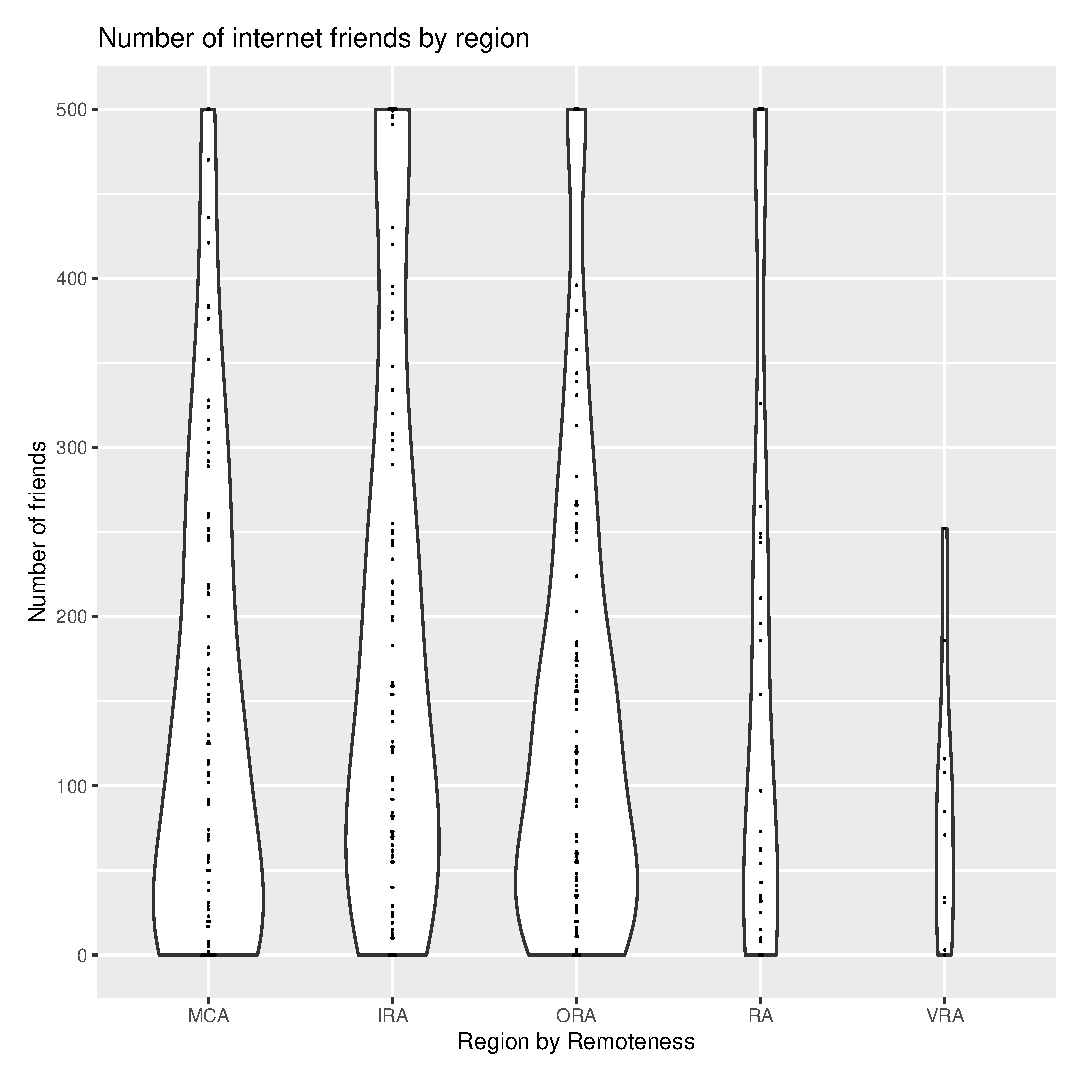
\includegraphics[scale=0.5]{figures/VChart16-NumberFriendsRegion.eps}
\caption{Survey Results - Average number of friends a person has by Region} \label{fig:VC016NumFriendsRegions}
\end{figure}
The number of `friends' a person makes on social media has an implication for their mental health. People with a large number of friends are correlated with being well socialised and supported by their friendship network. Facebook, for example, automatically attempts to increase the size of a person's group of friends based on the knowledge that people with fewer friends that 17 are unlikely to use the service. This would indicate that anyone with a group of friends over 17 is likely to receive reinforcement for using the Facebook service and therefore more likely to visit it regularly. Since regular repeat use is a key selling proposition of social network sites (SNS) it is in the interests of those sites to make interacting with connections a rewarding experience.

Research suggests that interacting with friends and making more friends on an SNS can increase social support. 

\begin{quotation}
People receive a range of different types of support on and off of the internet. They get
emotional support, such as advice; companionship, such as spending time with someone; and
more tangible support, such as help when they are sick. In our report on \emph{Social Network Sites
and Our Lives}, we found that internet users, and Facebook users in particular received more
social support --- not just online but from all their relationships combined.
In our survey, we measured support using the MOS Social Support Scale which included
measures of ``total support,'' ``emotional support,'' ``companionship,'' and ``instrumental aid.''
Activity logs of how people actually use Facebook provide further evidence of the positive
relationship between Facebook use and social support. Those
Facebook users who received more friend requests and accepted more of those friend requests
tended to report higher levels of total support. It is interesting to note that sending friend
request that were not reciprocated was not associated with more or less support\cite[p24]{RefWorks:364}.
\end{quotation}

Respondents to this survey were evenly distributed between no friends and 500 or more friends for Major Cities, Inner and Outer Regional Areas and even Remote Areas. In Very Remote Areas there was a striking halving of the number of friends reported by respondents. While there were only eight respondents in the Very Remote Area category, it is this category that is the most at risk of social isolation and it is this category and Remote Area respondents that stand to benefit from using the internet to remove that isolation. It may be that the number of friends a respondent connects with is smaller in Very Remote Areas because of the large geographical distance between their local community and their internet friends. A previous study of communications among users in a messaging network found that ``\ldots{} the total number of links and associated conversations decreases with increasing distance among participants. The same is true for the duration of conversations, the number of exchanged messages per conversation, and the number of exchanged messages per unit time\cite[p18]{RefWorks:319}.''





\section{Autonomous Device Networks}
Networking company CISCO has reported that, by 2021, there will be three times as many networked devices on the internet as there are people on the planet. Every individual using the internet is expected to have 3.5 networked devices where, in 2016, there were 2.3 networked devices per capita. Machine to machine (M2M) traffic is expected to have a Compound Annual Growth Rate (CAGR) of 45\% which is the same as the growth rate of smart phones\cite{RefWorks:346}.

This machine to machine traffic is generated by a range of devices that are mobile by nature such as cars, trucks, buses and non--mobile devices such as vending machines, power meters, parking meters, ATMs, remote sensors for agricultural and scientific uses, remote controls for equipment and machinery in farming applications. Using the mobile internet to send information removes the need for a telephone line rental and makes devices such as mobile contactless payment terminals portable in remote regions where a phone line would be impractical such as a local market, sporting event or 

Remote areas of Australia present issues for some of the latest automotive technology. Some new cars rely on connectivity to the mobile phone network. The car is immobilised until unlocked by a smart card or mobile phone app. Some drivers have found that they can lock themselves out of their Tesla cars if they don't have the right key on them and they have parked the car out of range of the mobile phone network. It is possible to unlock a Tesla car with a smart phone but if there is no mobile reception then the car cannot check back with the security profile held on file to verify if the smart phone being presented to the lock belongs to the cars owner or not. There have also been cases where car share cars, that require a smart card to unlock them, have become undriveable when switched off out of mobile range. The solution is to tow the vehicle back into range of the mobile network. 

Cars can also access `over the air' downloads of software, removing the need for them to visit a dealer or service station to have software patches applied to the control systems for the vehicle. Although there have been celebrated cases where cars have been `hacked' and either immobilised, having the facility to update vehicle software simultaneously over an entire fleet of vehicles means that security patches can be applied to prevent any exploit that may be devised over the entire fleet without haveing to organise an expensive recall by the manufacturer and without having to mail out software to owners for them to apply themselves using a USB stick loaded with the patch\cite{RefWorks:351}. 

Recently, telco, AT\&T had a profitable quarter but only because most of its new customers were the broadband modems inside new cars. These modems are part of a system in use in the United States and other countries where users can unlock their vehicle remotely if they lock the keys inside it or lose the keys. The driver calls a service centre and, after verifying ownership, a code is sent over the mobile network to the vehicle to unlock it. This service can also be used to call for help or roadside assistance by pressing a dedicated button inside the car. For electric vehicles, such as Tesla or Nissan Leaf, the mobile network can be used to check on the status of the car's battery while it is charging.  While many European countries have announced bans on non-electric vehicles being sold, it will be some time before electric vehicles will outnumber non--electric vehicles in Australia. This is due in part to the fact that the number of charging stations in Australia is very low and that they are mostly in urban areas. State governments in Queensland and Western Australia have announced plans for `electric highways' to ensure that there are enough charging stations on popular road routes to allow drivers to take electric vehicles for the same distances in a daily drive as non--electric vehicles.

In the past poor mobile service has been one reason that services that rely on a mobile connection in the car have been poorly received in Australia because the mobile network has made them unusable.


\begin{quotation}
Annual global IP traffic will reach 3.3 ZB (ZB; 1000 Exabytes [EB])
by 2021. In 2016, global IP traffic was 1.2 ZB per year or 96 EB (one billion
Gigabytes [GB]) per month. By 2021, global IP traffic will reach 3.3 ZB per
year, or 278 EB per month.

Global IP traffic will increase nearly threefold over the next 5 years, and
will have increased 127-fold from 2005 to 2021. Overall, IP traffic will grow
at a Compound Annual Growth Rate (CAGR) of 24 percent from 2016 to
2021.

Busy-hour Internet traffic is growing more rapidly than average Internet
traffic. Busy-hour (or the busiest 60 minute period in a day) Internet traffic
increased 51 percent in 2016, compared with 32-percent growth in average
traffic. Busy-hour Internet traffic will increase by a factor of 4.6 between
2016 and 2021, while average Internet traffic will increase by a factor of 3.2.

Smartphone traffic will exceed PC traffic by 2021. In 2016, PCs
accounted for 46 percent of total IP traffic, but by 2021 PCs will account for
only 25 percent of traffic. Smartphones will account for 33 percent of total
IP traffic in 2021, up from 13 percent in 2016. PC-originated traffic will grow
at a CAGR of 10 percent, while TVs, tablets, smartphones, and Machine-to-
Machine (M2M) modules will have traffic growth rates of 21 percent,
29 percent, 49 percent, and 49 percent, respectively.

Traffic from wireless and mobile devices will account for more than
63 percent of total IP traffic by 2021. By 2021, wired devices will account
for 37 percent of IP traffic, while Wi-Fi and mobile devices will account for
63 percent of IP traffic. In 2016, wired devices accounted for the majority of
IP traffic at 51 percent.

Global Internet traffic in 2021 will be equivalent to 127 times the volume
of the entire global Internet in 2005. Globally, Internet traffic will reach
30 GB per capita by 2021, up from 10 GB per capita in 2016.

The number of devices connected to IP networks will be three times as
high as the global population in 2021. There will be 3.5 networked devices
per capita by 2021, up from 2.3 networked devices per capita in 2016.
Accelerated in part by the increase in devices and the capabilities of those
devices, IP traffic per capita will reach 35 GB per capita by 2021, up from
13 GB per capita in 2016.

Broadband speeds will nearly double by 2021. By 2021, global fixed
broadband speeds will reach 53.0 Mbps, up from 27.5 Mbps in 2016.
\end{quotation}

Trillion Node Network\cite{RefWorks:321}
Scalability
Tractability

\subsection{Autonomous Machines and their effect on society}
\subsubsection{Robots}


\subsubsection{Autonomous cars}
Loss of work for delivery drivers and taxi drivers
Loss of work for Bus drivers and impact on round the clock transportation


\subsubsection{Autonomous trains}
Mining sector autonomous trains

Significant loss of jobs in remote and regional areas if implemented for all freight trains
\subsubsection{Autonomous Trucks}
Trucking is a significant industry in Australia employing [info needed] truck drivers in 2015.
Tesla working on Autonomous trucks, Tesla Semi, 
\subsubsection{Drone delivery}
Autonomous vehicles such as drones, cars or motorcycles could provide 24/7 deliveries in the future with higher reliability and less cost than existing human driven solutions. The Northern Sydney Local Health District has been considering using drones to deliver time critical blood products at a fraction of the cost of deploying a helicopter for the same service.\cite{RefWorks:409} The mission parameters of delivering medication to the remotest areas of Australia are similar to the missions flown by the Royal Flying Doctor but drone delivery does not require an air field or expensive airplanes with several people crewing each mission for each delivery. Rather than tens of thousands of dollars per mission, deliveries can be organised by doctors or patients themselves through text or web portals for hundreds of dollars. Drone delivery is cost competitive with existing courier delivery but while a courier may take hours or even a day to deliver time critical medical supplies, drone delivery can often achieve the same effect in under an hour. 

\begin{quotation}
One application where drone delivery may make more sense, and is already in use, is ferrying medical supplies to remote areas that are hard to reach by road. Zipline, an American startup staffed by veterans of Google, SpaceX, Boeing and NASA, began delivering medical supplies in rural Rwanda using fixed-wing drones in October 2016. It has an agreement with the government to deliver blood products to 21 transfusion clinics from two bases, the first of which is already serving five clinics. Zipline's drones can fly 150km on a single charge and work in rain and winds of up to 30km an hour. They are launched using a catapult, fly below 150 metres (500 feet) and drop cargo packages weighing 1.5kg by parachute\cite{RefWorks:350}.

\end{quotation}
While drone delivery is currently competitive for the delivery of time critical medical supplies, as the technology is perfected it is reasonable to assume that drone delivery will take the place of many deliveries that are currently performed by couriers or postal workers. Amazon is pursuing drone delivery with its Amazon Prime initiative and has conducted proof of concept deliveries as have other companies such as Australian startup, Flirty, now based in the USA\cite{RefWorks:411}.

\subsubsection{Drone surveillance}
Drone surveillance is important in Australia where large geographical areas must be under surveillance for national, state and local security purposes as well as for economic reasons.
Power lines, pipelines, wind turbines, oil rigs and electricity lines need regular inspection and when this is done by drone, more reliable infrastructure results due to faster mean time to repair and through preventative maintenance which makes these machinery and transportation networks more reliable. [citation needed]


